\documentclass[a4paper, 11pt] {article}

\usepackage[utf8]{inputenc}
\usepackage[T1, T2A]{fontenc}
\usepackage[english, russian]{babel}
\usepackage{graphicx}
\usepackage[top=2cm, left=2cm, right=2cm, left=2cm]{geometry}
\usepackage{amsmath}
\newcommand\tline[2]{$\underset{\text{#1}}{\text{\underline{\hspace{#2}}}}$}

\begin{document}
	\begin{titlepage}
		\centering
		{\fontsize{12pt}{5cm}\selectfont \bfseries Министерство образования и науки Российской Федерации} \\ \vspace{0.5cm}
		{\fontsize{7pt}{5cm}\selectfont ФЕДЕРАЛЬНОЕ ГОСУДАРСТВЕННОЕ АВТОНОМНОЕ ОБРАЗОВАТЕЛЬНОЕ УЧРЕЖДЕНИЕ ВЫСШЕГО ПРОФЕССИОНАЛЬНОГО ОБРАЗОВАНИЯ} \\ 
		\vspace{1cm}
		{\fontsize{12pt}{5cm}\selectfont \bfseries САНКТ-ПЕТЕРБУРГСКИЙ УНИВЕРСИТЕТ ИНФОРМАЦИОННЫХ ТЕХНОЛОГИЙ, МЕХАНИКИ И ОПТИКИ} \\ \vspace{1.5cm}

		{\fontsize{14pt}{5cm}\selectfont Кафедра \hspace{1cm} \underline{Систем Управления и Информатики}  \hspace{1cm} Группа \underline{Р3340}} \\ 
		\vspace{2cm}

		{\fontsize{20pt}{5cm}\selectfont \bfseries Лабораторная работа №8} \\
		{\fontsize{12pt}{5cm}\selectfont \bfseries “ЭКСПЕРИМЕНТАЛЬНОЕ ПОСТРОЕНИЕ ОБЛАСТЕЙ
			УСТОЙЧИВОСТИ ЛИНЕЙНОЙ СИСТЕМЫ НА ПЛОСКОСТИ
			ДВУХ ПАРАМЕТРОВ
			”} \\
		{\fontsize{14pt}{5cm}\selectfont Вариант - 11} \\
		\vspace{1.5cm}

		\flushleft

		{Выполнил \hspace{2cm}\underline{Та М.Ш}\tline{(фамилия, и.о.)}{9cm} (подпись)} \\
		\vspace{2cm}

		{Проверил \hspace{2cm} \tline{(фамилия, и.о.)}{9cm} (подпись)} \\
		\vspace{5cm}

		"\underline{\hspace{0.7cm}}"\hspace{0.2cm}\underline{\hspace{2cm}}\hspace{0.2cm}20\underline{\hspace{0.7cm}}г. \hspace{2cm} Санкт-Петербург, \hspace{2cm} 20\underline{\hspace{0.7cm}}г. \\ \vspace{1cm}

		Работа выполнена с оценкой \hspace{1cm} \underline{\hspace{8cm}} \\ 
		\vspace{1cm}
		Дата защиты "\underline{\hspace{0.7cm}}"\hspace{0.2cm}\underline{\hspace{2cm}}\hspace{0.2cm}20\underline{\hspace{0.7cm}}г.

	\end{titlepage}

\section*{Цель работы}
Ознакомление с экспериментальными методами построения областей устойчивости линейных динамических систем и изучение влияния на устойчивость системы ее параметров.

\section{Собрать схему моделирования, установив значение постоянной времени}


\begin{figure}[h]
	\centering
	\center{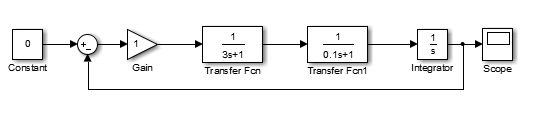
\includegraphics[width=0.7\linewidth]{0.png}}
	\caption{Схема моделирования}
	\label{fig:0}
\end{figure}

\begin{figure}[h]
	\centering
	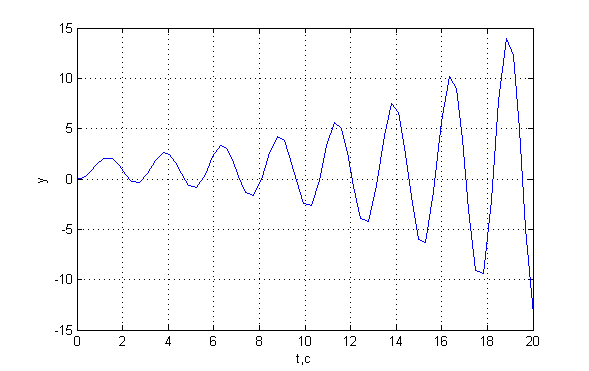
\includegraphics[width=0.7\linewidth]{1}
	\caption{Графика неустойчивости САУ}
	\label{fig:1}
\end{figure}

\begin{figure}[h]
	\centering
	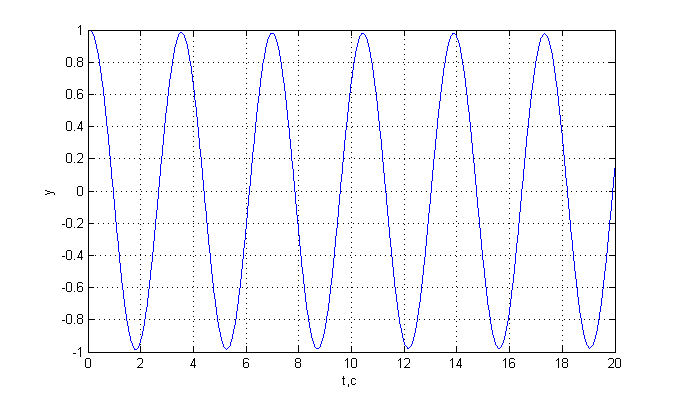
\includegraphics[width=0.7\linewidth]{2}
	\caption{Графика САУ на границе устойчивости}
	\label{fig:2}
\end{figure}

\begin{center}
	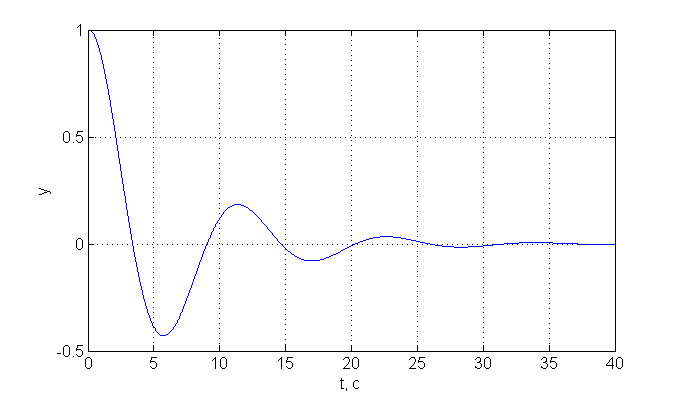
\includegraphics[width=0.7\linewidth]{3}
\begin{figure}[h]
		\caption{Графика устойчивости САУ}
	\label{fig:3}
\end{figure}
\end{center}

\section{Построим экспериментальную границу устойчивости}
\begin{center}
\begin{tabular}{|c|c|c|c|c|c|c|c|c|c|c|c|}
	\hline 
	T2 & 0.1 & 0.5 & 1 & 1.5 & 2 & 2.5 & 3 & 3.5 & 4 & 4.5 & 5 \\ 
	\hline 
	K & 10.3 & 2.3 & 1.3 & 1 & 0.83 & 0.73 & 0.67 & 0.62 & 0.58 & 0.55 & 0.53 \\ 
	\hline 
\end{tabular} 
\end{center}
\section{Теоретический расчет границы устойчивости с использованием критерия Гурвица}

% MathType!MTEF!2!1!+-
% feaagGart1ev2aaatCvAUfeBSjuyZL2yd9gzLbvyNv2CaerbuLwBLn
% hiov2DGi1BTfMBaeXatLxBI9gBaerbd9wDYLwzYbItLDharqqtubsr
% 4rNCHbGeaGqiVu0Je9sqqrpepC0xbbL8F4rqqrFfpeea0xe9Lq-Jc9
% vqaqpepm0xbba9pwe9Q8fs0-yqaqpepae9pg0FirpepeKkFr0xfr-x
% fr-xb9adbaqaaeGaciGaaiaabeqaamaabaabaaGcbaGaam4vaiaacI
% cacaWGZbGaaiykaiabg2da9maalaaabaGaaiikaiaaiodacaWGZbGa
% ey4kaSIaaGymaiaacMcacaGGOaGaaiivamaaBaaaleaacaaIYaaabe
% aakiaadohacqGHRaWkcaaIXaGaaiykaiaacohaaeaacaGGOaGaaG4m
% aiaadohacqGHRaWkcaaIXaGaaiykaiaacIcacaGGubWaaSbaaSqaai
% aaikdaaeqaaOGaam4CaiabgUcaRiaaigdacaGGPaGaam4CaiabgUca
% RiaadUgaaaaaaa!52BF!
    Передаточная функция  \[W(s) = \frac{{(3s + 1)({T_2}s + 1)s}}{{(3s + 1)({T_2}s + 1)s + k}}\]
% MathType!MTEF!2!1!+-
% feaagGart1ev2aaatCvAUfeBSjuyZL2yd9gzLbvyNv2CaerbuLwBLn
% hiov2DGi1BTfMBaeXatLxBI9gBaerbd9wDYLwzYbItLDharqqtubsr
% 4rNCHbGeaGqiVu0Je9sqqrpepC0xbbL8F4rqqrFfpeea0xe9Lq-Jc9
% vqaqpepm0xbba9pwe9Q8fs0-yqaqpepae9pg0FirpepeKkFr0xfr-x
% fr-xb9adbaqaaeGaciGaaiaabeqaamaabaabaaGceaqabeaacaGGOa
% GaaG4maiaadohacqGHRaWkcaaIXaGaaiykaiaacIcacaGGubWaaSba
% aSqaaiaaikdaaeqaaOGaam4CaiabgUcaRiaaigdacaGGPaGaam4Cai
% abgUcaRiaadUgacqGH9aqpcaaIWaaabaGaeyi1HSTaaG4maiaadsfa
% daWgaaWcbaGaaGOmaaqabaGccaWGZbWaaWbaaSqabeaacaaIZaaaaO
% Gaey4kaSIaaiikaiaaiodacqGHRaWkcaWGubWaaSbaaSqaaiaaikda
% aeqaaOGaaiykaiaadohadaahaaWcbeqaaiaaikdaaaGccqGHRaWkca
% WGZbGaey4kaSIaam4Aaiabg2da9iaaicdaaaaa!58B5!
\[\begin{array}{l}
(3s + 1)({T_2}s + 1)s + k = 0\\
\Leftrightarrow 3{T_2}{s^3} + (3 + {T_2}){s^2} + s + k = 0
\end{array}\]

Матрица Гурвицы % MathType!MTEF!2!1!+-
% feaagGart1ev2aaatCvAUfeBSjuyZL2yd9gzLbvyNv2CaerbuLwBLn
% hiov2DGi1BTfMBaeXatLxBI9gBaerbd9wDYLwzYbItLDharqqtubsr
% 4rNCHbGeaGqiVu0Je9sqqrpepC0xbbL8F4rqqrFfpeea0xe9Lq-Jc9
% vqaqpepm0xbba9pwe9Q8fs0-yqaqpepae9pg0FirpepeKkFr0xfr-x
% fr-xb9adbaqaaeGaciGaaiaabeqaamaabaabaaGcbaGaamyqaiabg2
% da9maabmaabaqbaeqabiGaaaqaaiaaiodacqGHRaWkcaWGubWaaSba
% aSqaaiaaikdaaeqaaaGcbaGaam4AaaqaaiaaiodacaWGubWaaSbaaS
% qaaiaaikdaaeqaaaGcbaGaaGymaaaaaiaawIcacaGLPaaaaaa!40F7!
\[A = \left( {\begin{array}{*{20}{c}}
	{3 + {T_2}}&k\\
	{3{T_2}}&1
	\end{array}} \right)\]
САУ устойчивость на границе когда % MathType!MTEF!2!1!+-
% feaagGart1ev2aaatCvAUfeBSjuyZL2yd9gzLbvyNv2CaerbuLwBLn
% hiov2DGi1BTfMBaeXatLxBI9gBaerbd9wDYLwzYbItLDharqqtubsr
% 4rNCHbGeaGqiVu0Je9sqqrpepC0xbbL8F4rqqrFfpeea0xe9Lq-Jc9
% vqaqpepm0xbba9pwe9Q8fs0-yqaqpepae9pg0FirpepeKkFr0xfr-x
% fr-xb9adbaqaaeGaciGaaiaabeqaamaabaabaaGcbaGaeyiLdqKaey
% ypa0JaaiikaiaaiodacqGHRaWkcaWGubWaaSbaaSqaaiaaikdaaeqa
% aOGaaiykaiabgkHiTiaaiodacaWGubWaaSbaaSqaaiaaikdaaeqaaO
% Gaam4Aaiabg2da9iaaicdaaaa!434A!
\[\Delta  = (3 + {T_2}) - 3{T_2}k = 0\]
% MathType!MTEF!2!1!+-
% feaagGart1ev2aaatCvAUfeBSjuyZL2yd9gzLbvyNv2CaerbuLwBLn
% hiov2DGi1BTfMBaeXatLxBI9gBaerbd9wDYLwzYbItLDharqqtubsr
% 4rNCHbGeaGqiVu0Je9sqqrpepC0xbbL8F4rqqrFfpeea0xe9Lq-Jc9
% vqaqpepm0xbba9pwe9Q8fs0-yqaqpepae9pg0FirpepeKkFr0xfr-x
% fr-xb9adbaqaaeGaciGaaiaabeqaamaabaabaaGcbaGaam4Aaiabg2
% da9maalaaabaGaaG4maiabgUcaRiaadsfadaWgaaWcbaGaaGOmaaqa
% baaakeaacaaIZaGaamivamaaBaaaleaacaaIYaaabeaaaaaaaa!3DE3!
\[k = \frac{{3 + {T_2}}}{{3{T_2}}}\]

\begin{figure}[ht]
	\centering
	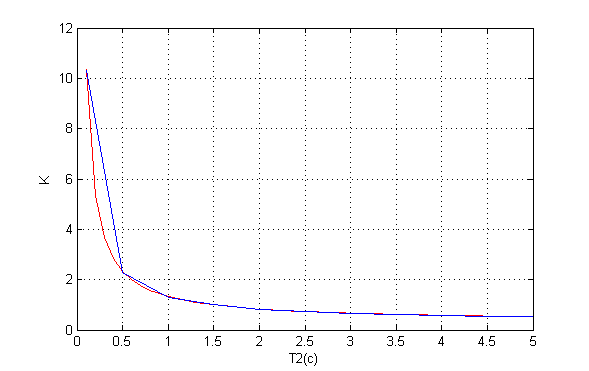
\includegraphics[width=0.7\linewidth]{4}
	\caption{Графика границы устойчивости САУ}
	\label{fig:4}
\end{figure}

\section*{Выводы}
При проектировании систем большое значение имеет определение областей устойчивости в плоскости реальных параметров, присущих системе. Система является устойчивой ,соответственно, множество значений параметров находится ниже границы устойчивости (при % MathType!MTEF!2!1!+-
% feaagGart1ev2aaatCvAUfeBSjuyZL2yd9gzLbvyNv2CaerbuLwBLn
% hiov2DGi1BTfMBaeXatLxBI9gBaerbd9wDYLwzYbItLDharqqtubsr
% 4rNCHbGeaGqiVu0Je9sqqrpepC0xbbL8F4rqqrFfpeea0xe9Lq-Jc9
% vqaqpepm0xbba9pwe9Q8fs0-yqaqpepae9pg0FirpepeKkFr0xfr-x
% fr-xb9adbaqaaeGaciGaaiaabeqaamaabaabaaGcbaGaam4saiabgs
% MiJoaalaaabaGaaG4maiabgUcaRiaadsfadaWgaaWcbaGaaGOmaaqa
% baaakeaacaaIZaGaamivamaaBaaaleaacaaIYaaabeaaaaaaaa!3E72!
\ k \le \frac{{3 + {T_2}}}{{3{T_2}}}\)
\end{document}